\scanpage{39}

$X$ propre et simple sur $k$ [\unsure{généraliser|généralisons} à une base quelconque]

$A$ V.A. sur $k$

$H^1(X,A)=\underset{n}{\varinjlim}\ {}_nH^1(X,A)$ \begin{tikzpicture}[x=1ex,y=1ex,baseline=0pt]
\fill (0,.35)--(.03,.53)--(.23,.59)--(.27,.72)--(.41,.66)--(.48,.7)--(.55,.62)--(.78,.58)--(.92,.46)--(.95,.23)--(.87,.25)--(.84,.36)--(.64,.38)--(.35,.36)--cycle;
\fill (.14,.04) ellipse (.055 and .05);
\end{tikzpicture} d'autre part on a une suite exacte
\diagram{\begin{tikzcd}[ampersand replacement=\&, column sep=small]
0 \arrow[r] \& \operatorname{Hom}(X,A)_n \arrow[r] \& {}_{\deleted{\unsure{n}}}H^1(X,{}_nA) \arrow[r] \& {}_nH^1(X,A) \arrow[r] \& 0
\end{tikzcd}}
qui s'écrit aussi
\diagram{\begin{tikzcd}[ampersand replacement=\&, column sep=small]
0 \arrow[r] \& \operatorname{Hom}(\operatorname{Alb}_X,A)_n \arrow[r] \& \operatorname{Hom}(D({}_nA),\operatorname{Pic}_X) \arrow[r] \& {}_nH^1(X,A) \arrow[r] \& 0
\end{tikzcd}}

\unsure{en effet}, cela par
\par\noindent\hspace*{0.51\linewidth}$\unsure{l|1}$
\[
\operatorname{Hom}(\operatorname{Alb}_X,A)\simeq\operatorname{Hom}(A',(\operatorname{Alb}_X)')=\operatorname{Hom}(A',\operatorname{Pic}_X^0)
\]
\[
D({}_nA)\simeq{}_nA'
\]
une suite exacte

$(*)$
\diagram{\begin{tikzcd}[ampersand replacement=\&, column sep=small]
0 \arrow[r] \& \operatorname{Hom}(A',\operatorname{Pic}_X^{\unsure{0|\tau}})_n \arrow[r] \& \operatorname{Hom}({}_{\unsure{n}}A',\operatorname{Pic}_X) \arrow[r] \& {}_nH^1(X,A) \arrow[r] \& 0
\end{tikzcd}}
et passant à la limite
\begin{tabular}[b]{@{}l@{}}
\hspace{0.3em}\inserted{\unsure{inductive}}\\[0.5ex]
\rlap{\begin{tikzpicture}[x=1em,y=1ex,baseline=0pt,overlay]
\draw[->,line width=0.35pt] (-0.2,-0.4) .. controls (-0.3,1.6) and (0.8,1.8) .. (2.1,1.8) .. controls (3.8,1.6) and (4.6,1.7) .. (5.1,2.3);
\end{tikzpicture}}sur $n$ :
\end{tabular}
\diagram{\begin{tikzcd}[ampersand replacement=\&, column sep=small,
execute at end picture={
\draw[line width=0.35pt] ([xshift=-0.6em,yshift=0.8ex]\tikzcdmatrixname.north west) -- ([xshift=0.25em,yshift=1.7ex]\tikzcdmatrixname.north east) .. controls ([xshift=.38em,yshift=1.7ex]\tikzcdmatrixname.north east) and ([xshift=.45em,yshift=1.55ex]\tikzcdmatrixname.north east) .. ([xshift=.5em,yshift=1.55ex]\tikzcdmatrixname.north east);
\draw[line width=0.35pt] ([xshift=-0.6em,yshift=-0.1ex]\tikzcdmatrixname.north west) -- ([xshift=-0.5em,yshift=-0.7ex]\tikzcdmatrixname.south west) -- ([xshift=0.3em,yshift=0ex]\tikzcdmatrixname.south east) .. controls ([xshift=.4em,yshift=0ex]\tikzcdmatrixname.south east) and ([xshift=.46em,yshift=.08ex]\tikzcdmatrixname.south east) .. ([xshift=.5em,yshift=.12ex]\tikzcdmatrixname.south east);
}]
0 \arrow[r] \& \operatorname{Hom}(A',\underline{\operatorname{Pic}}_X^{\unsure{0|\tau}})\otimes_{\mathbb Z}\mathbb Q \arrow[r] \& \operatorname{Hom}(T_{\cdot}(A'),\underline{\operatorname{Pic}}_X) \arrow[r] \& H^1(X,A) \arrow[r] \& 0
\end{tikzcd}}

Or la suite exacte $(*)$ se compare à la suite exacte déduite de
\diagram{\begin{tikzcd}[ampersand replacement=\&, column sep=small]
0 \arrow[r,no head] \& {}_n\unsure{A|\Lambda}' \arrow[r,no head] \& A' \arrow[r] \& A' \arrow[r] \& 0
\end{tikzcd}}
en appliquant $\deleted{\operatorname{Ext}^{\unsure{1}}}\underline{\operatorname{Hom}}(-,\operatorname{Pic}_X)$, on \unsure{trouve}

$(*\unsure{*|+})$
\diagram{\begin{tikzcd}[ampersand replacement=\&, column sep=small]
0 \arrow[r,no head] \& \operatorname{Hom}(A',\underline{\operatorname{Pic}}_X)_n \arrow[r] \& \operatorname{Hom}({}_{\unsure{n}}A',\underline{\operatorname{Pic}}_X) \arrow[r] \& {}_n\operatorname{Ext}^1(A',\underline{\operatorname{Pic}}_X^{\unsure{\tau|2}}) \arrow[r] \& 0
\end{tikzcd}}
qui donne à la limite
\diagram{\begin{tikzcd}[ampersand replacement=\&, column sep=small,row sep=tiny,
execute at end picture={
\draw[line width=0.35pt] ([xshift=-0.6em,yshift=0.8ex]\tikzcdmatrixname.north west) -- ([xshift=0.25em,yshift=1.2ex]\tikzcdmatrixname.north east) .. controls ([xshift=.4em,yshift=1.2ex]\tikzcdmatrixname.north east) and ([xshift=.46em,yshift=1.08ex]\tikzcdmatrixname.north east) .. ([xshift=.5em,yshift=1.04ex]\tikzcdmatrixname.north east);
\draw[line width=0.35pt] ([xshift=-0.6em,yshift=-0.1ex]\tikzcdmatrixname.north west) -- ([xshift=-0.6em,yshift=-0.6ex]\tikzcdmatrixname.south west) -- ([xshift=0.5em,yshift=-0.7ex]\tikzcdmatrixname.south east);
}]
0 \arrow[r,no head] \& \operatorname{Hom}(A',\operatorname{Pic}_X)\otimes_{\mathbb Z}\mathbb Q \arrow[r] \& \operatorname{Hom}(T_{\cdot}(A'),\operatorname{Pic}_X) \arrow[r,no head] \& \operatorname{Ext}^1(A',\underline{\operatorname{Pic}}_X) \arrow[dr,bend left=15] \& \\
 \& \& \& \& \unsure{0}
\end{tikzcd}}
\margin{38}
